
% \part{Theory}

\section{Single Particle Dynamics}
\label{sec:single_particle_dynamics}

Equations of motion for charged particles under the effects of accelerator
components, such as dipoles and quadrupoles, can be derived through the
application of Maxwell's equations \cite{}. The solutions to these equations
become increasingly complex at higher perturbations so it is usefull to devise
a system from which we are ???

Specifying a coorindate system such that the origin follows the ideal path of
the particle beam, rather than a coordinate system about an arbitary fixed
point we are able to describe the state of a patricle by

\begin{equation}
	\begin{pmatrix}
		x(z) \\ x'(z) \\
		y(z) \\ y'(z) \\
	\end{pmatrix}
	=
	\begin{pmatrix}
		C_x(z)  & S_x(z)  & 0 & 0 \\
		C'_x(z) & S'_x(z) & 0 & 0 \\
		0 & 0 & C_y(z)  & S_y(z)  \\
		0 & 0 & C'_y(z) & S'_y(z) \\
	\end{pmatrix}
	\begin{pmatrix}
		x_0 \\ x'_0 \\
		y_0 \\ y'_0 \\
	\end{pmatrix}
\end{equation}

where \(x\) and \(y\) are deviations form the centre of the beam along their
respective axis and \(x'\) and \(y'\) are the transverse momenta of the
particle perpendicular to \(z\), the direction of travel of the beam.
Transformations in either the $x$ or $y$ plane are independent, however, it is
clear that coupling effects can still be included
% TODO




\section{Emittance}

The beam emittance is a
% quantity that describes the collective motion of all the particles in the
% beam, providing a
qualitative way of describing the quality of the beam, essentially, it is a
measure of how parallel the particles of the beam are to each other.
It is a conserved
quantity in the absence of a \(z\) component (i.e. in the direction of the
beam) in the magnetic field and when the beam is not being accelerated.

The position of each particle in Cartesian coordinates is not sufficient in
describing the state of a beam so each beam particle is represented in
six-dimensional phase space with coordinates \(\left(x,p_x,y,p_y,z,p_z\right)\)
where \(p_x\approx~p_0x'\) and \(p_y\approx~p_0y'\) are the transverse momenta,
\(z\) is the position along the beam trajectory, \(p_z\) is the longitudinal
momentum and \(x'\) and \(y'\) are the trajectory angles to the horizontal and
vertical planes. Since the transverse momenta, and therefore \(x'\) and \(y'\),
are generally quite small we can approximate \(\sin\left(x'\right)\approx x'\)
and \(\sin\left(y'\right)\approx y'\). We can then project this six-dimensional
volume into three independent two-dimensional phase planes, because in this
approximation there is no coupling between those degrees of freedom.

The horizontal emittance of the beam is defined by considering the ellipse in
the \(x'-x\) phase space that contains \(95\%\) of all the
particles~\cite{buon1994beam}. The area contained by this ellipse divided by
\(\pi\) is defined as the emittance in units of \(\pi\)-mm-mrad.

\[ \int_{\text{ellipse}}\mathrm{d}x\mathrm{d}x' =\pi\epsilon \]

\begin{figure}[!t]
	\centering
	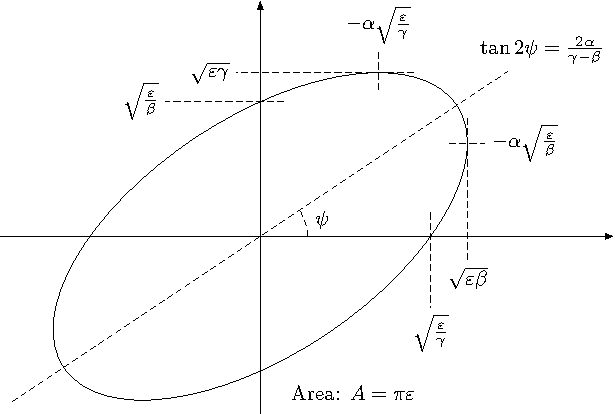
\includegraphics{figures/ellipse}
	\caption{
		Graphical representation of the relation between the twiss parameters
		\cite{caldwell2015rkk}}
	\label{fig:ellipse}
\end{figure}

Fig. \ref{fig:ellipse} shows a beam projected onto a two dimensional phase
plane. The emittance can be described by the equation of the ellipse:

\[ \gamma x^2 + 2\alpha xx' + \beta x'^2 = \epsilon \]

where \(\alpha\),  \(\beta\) are \(\gamma\) are ellipse parameters that
determine the ellipse's shape and orientation and are related by this equation

\[ \beta\gamma - \alpha^2 = 1 \]

% \subsection{Methods of measurement}

% The phase-space density and emittance of a beam must be infered from beam
% profiles captured using charge-coupled device (CCD) cameras after undergoing
% spatial filtering.

It follows that the beam matrix is

\[\sigma =
	\begin{pmatrix}
	  \sigma_{1,1} & \sigma_{1,2} \\
	  \sigma_{2,1} & \sigma_{2,2} \\
	\end{pmatrix}
	=
	\begin{pmatrix}
	  \beta\epsilon^2 & -\alpha\epsilon^2 \\
	  -\alpha\epsilon^2 & \gamma\epsilon^2 \\
	\end{pmatrix}
\]

such that \(\epsilon = \det\sigma\), \(\sigma_{1,1}\) is the besm size and
\(\sigma_{1,2}\) is the orientation in phase space. We can relate the beam
matrix after passing through quadrupoles, \(\sigma_1\), to the original beam
matrix, \(\sigma_0\), as follows

\[
	\sigma_{1,11} = c^2(k)\sigma_{0,11} + 2c(k)s(k)\sigma_{0,12} +
	s^2(k)\sigma_{0,22}
\]

where we plot the final beam size \(\sigma_1,11\) against the quadrupole
strength \(k\).  \(\sigma_0\) is determined from the fit and it's determinant
will then give the emittance.

